\documentclass[11pt,letterpaper]{article}

% ============================================================================
% PACKAGES
% ============================================================================
\usepackage[utf8]{inputenc}
\usepackage[T1]{fontenc}
\usepackage[margin=1in]{geometry}
\usepackage{graphicx}
\usepackage{xcolor}
\usepackage{hyperref}
\usepackage{titlesec}
\usepackage{enumitem}
\usepackage{booktabs}
\usepackage{longtable}
\usepackage{tabularx}
\usepackage{multirow}
\usepackage{colortbl}
\usepackage{fancyhdr}
\usepackage{tocloft}
\usepackage{parskip}
\usepackage{tikz}
\usepackage{float}
\usepackage{framed}
\usepackage{mdframed}

% ============================================================================
% COLOR DEFINITIONS
% ============================================================================
\definecolor{primaryblue}{RGB}{0,82,147}
\definecolor{secondaryblue}{RGB}{51,122,183}
\definecolor{accentgold}{RGB}{218,165,32}
\definecolor{darkgray}{RGB}{64,64,64}
\definecolor{lightgray}{RGB}{245,245,245}
\definecolor{successgreen}{RGB}{40,167,69}
\definecolor{warningorange}{RGB}{255,140,0}

% ============================================================================
% HYPERREF SETUP
% ============================================================================
\hypersetup{
    colorlinks=true,
    linkcolor=primaryblue,
    filecolor=primaryblue,
    urlcolor=secondaryblue,
    citecolor=primaryblue,
    pdftitle={Enterprise Architecture Comprehensive Curriculum},
    pdfauthor={Professional Development Program},
    pdfsubject={Enterprise Architecture Education},
    pdfkeywords={Enterprise Architecture, Software Architecture, IT Strategy, Business Alignment},
    hypertexnames=false
}

% ============================================================================
% TITLE FORMATTING
% ============================================================================
\titleformat{\section}
{\color{primaryblue}\normalfont\Large\bfseries}
{\thesection}{1em}{}[\titlerule]

\titleformat{\subsection}
{\color{secondaryblue}\normalfont\large\bfseries}
{\thesubsection}{1em}{}

\titleformat{\subsubsection}
{\color{darkgray}\normalfont\normalsize\bfseries}
{\thesubsubsection}{1em}{}

% ============================================================================
% HEADER/FOOTER
% ============================================================================
\setlength{\headheight}{14pt}
\addtolength{\topmargin}{-2pt}
\pagestyle{fancy}
\fancyhf{}
\fancyhead[L]{\textcolor{darkgray}{\small Enterprise Architecture Curriculum}}
\fancyhead[R]{\textcolor{darkgray}{\small Professional Development Program}}
\fancyfoot[C]{\textcolor{darkgray}{\thepage}}
\renewcommand{\headrulewidth}{0.4pt}
\renewcommand{\footrulewidth}{0.4pt}

% ============================================================================
% CUSTOM ENVIRONMENTS
% ============================================================================
\newmdenv[
    backgroundcolor=lightgray,
    linecolor=primaryblue,
    linewidth=2pt,
    topline=false,
    bottomline=false,
    rightline=false,
    innertopmargin=10pt,
    innerbottommargin=10pt,
    innerrightmargin=10pt,
    innerleftmargin=15pt
]{keyconceptbox}

\newmdenv[
    backgroundcolor=white,
    linecolor=successgreen,
    linewidth=2pt,
    roundcorner=5pt,
    innertopmargin=10pt,
    innerbottommargin=10pt,
    innerrightmargin=10pt,
    innerleftmargin=10pt
]{learningoutcomebox}

\newmdenv[
    backgroundcolor=white,
    linecolor=warningorange,
    linewidth=2pt,
    roundcorner=5pt,
    innertopmargin=10pt,
    innerbottommargin=10pt
]{practicalexercisebox}

% ============================================================================
% CUSTOM COMMANDS
% ============================================================================
\newcommand{\bookref}[2]{\textit{#1} by #2}
\newcommand{\duration}[1]{\textcolor{secondaryblue}{$\triangleright$ Duration: #1}}
\newcommand{\difficulty}[1]{\textcolor{warningorange}{Level: #1}}
\newcommand{\prereq}[1]{\textcolor{successgreen}{Prerequisites: #1}}

% ============================================================================
% DOCUMENT BEGINS
% ============================================================================
\begin{document}

% ============================================================================
% TITLE PAGE
% ============================================================================
\begin{titlepage}
    \centering
    \vspace*{1.5cm}
    
    {\color{primaryblue}\rule{\linewidth}{2pt}}
    
    \vspace{1cm}
    
    {\Huge\bfseries\color{primaryblue} Enterprise Architecture\\[0.5cm] Comprehensive Curriculum}
    
    \vspace{0.5cm}
    
    {\color{primaryblue}\rule{\linewidth}{2pt}}
    
    \vspace{1.5cm}
    
    {\Large\color{darkgray} A Professional Development Program for\\[0.3cm] Software Engineers Transitioning to Enterprise Architecture}
    
    \vspace{2cm}
    
    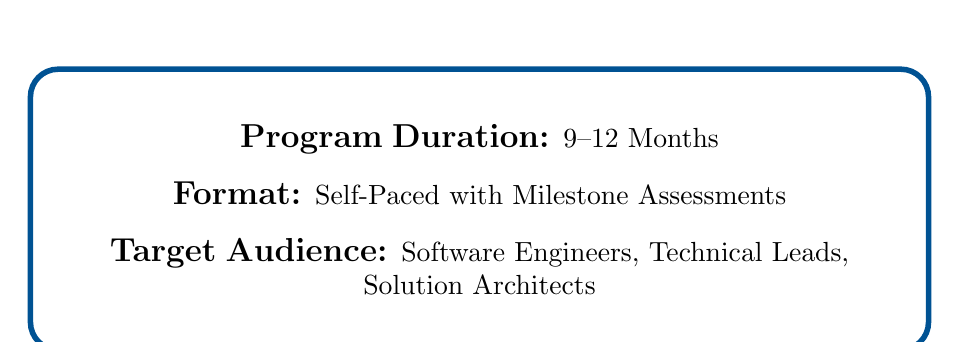
\begin{tikzpicture}
        \node[draw=primaryblue, line width=2pt, rounded corners=10pt, 
              inner sep=20pt, text width=10cm, align=center] {
            \textbf{\large Program Duration:} 9--12 Months\\[0.3cm]
            \textbf{\large Format:} Self-Paced with Milestone Assessments\\[0.3cm]
            \textbf{\large Target Audience:} Software Engineers, Technical Leads,\\
            Solution Architects
        };
    \end{tikzpicture}
    
    \vfill
    
    {\large\color{darkgray} Version 1.0}\\[0.3cm]
    {\large\color{darkgray} \today}
    
    \vspace{1cm}
\end{titlepage}

% ============================================================================
% TABLE OF CONTENTS
% ============================================================================
\tableofcontents
\newpage

% ============================================================================
% PROGRAM OVERVIEW
% ============================================================================
\section{Program Overview}

\subsection{Executive Summary}

This comprehensive curriculum is designed for software engineers and technical professionals seeking to transition into Enterprise Architecture (EA) roles. The program synthesizes theoretical foundations with practical application, drawing from the most influential texts in the field while emphasizing real-world implementation.

Enterprise Architecture is not merely an IT diagramming exercise---it is a strategic business discipline that bridges technology capabilities with organizational objectives. This curriculum prepares practitioners to operate effectively across all organizational levels, from the ``engine room'' of technical implementation to the ``penthouse'' of executive strategy.

\subsection{Program Objectives}

Upon completion of this curriculum, participants will be able to:

\begin{learningoutcomebox}
\textbf{Strategic Competencies}
\begin{itemize}[leftmargin=*]
    \item Articulate the business value of Enterprise Architecture to executive stakeholders
    \item Design operating models that align IT capabilities with business strategy
    \item Evaluate and select appropriate EA frameworks for organizational contexts
    \item Create governance structures that enable architectural evolution
\end{itemize}
\end{learningoutcomebox}

\begin{learningoutcomebox}
\textbf{Technical Competencies}
\begin{itemize}[leftmargin=*]
    \item Apply enterprise application patterns to system design
    \item Design integration architectures using proven messaging patterns
    \item Structure applications for testability, maintainability, and scalability
    \item Create architectural documentation that serves multiple stakeholder audiences
\end{itemize}
\end{learningoutcomebox}

\begin{learningoutcomebox}
\textbf{Organizational Competencies}
\begin{itemize}[leftmargin=*]
    \item Navigate organizational politics and change management
    \item Design team structures that support target architectures (Conway's Law)
    \item Communicate effectively with technical and non-technical stakeholders
    \item Lead architecture review boards and governance processes
\end{itemize}
\end{learningoutcomebox}

\subsection{Target Audience}

This curriculum is designed for professionals who meet the following criteria:

\begin{keyconceptbox}
\textbf{Primary Audience:}
\begin{itemize}[leftmargin=*]
    \item Software Engineers with 5+ years of development experience
    \item Technical Leads seeking to expand their architectural perspective
    \item Solution Architects transitioning to enterprise-level roles
    \item IT Managers responsible for technology strategy
\end{itemize}

\textbf{Prerequisites:}
\begin{itemize}[leftmargin=*]
    \item Proficiency in at least one programming language
    \item Experience with software development methodologies (Agile, Waterfall)
    \item Familiarity with database design and data modeling concepts
    \item Basic understanding of networking and distributed systems
    \item Experience participating in architectural discussions or reviews
\end{itemize}
\end{keyconceptbox}

\subsection{Curriculum Structure}

The curriculum is organized into four progressive phases, each building upon the previous:

\begin{table}[H]
\centering
\begin{tabularx}{\textwidth}{|c|X|c|c|}
\hline
\rowcolor{primaryblue}
\textcolor{white}{\textbf{Phase}} & \textcolor{white}{\textbf{Focus Area}} & \textcolor{white}{\textbf{Duration}} & \textcolor{white}{\textbf{Modules}} \\
\hline
I & Foundational \& Strategic Enterprise Architecture & 8--10 weeks & 3 \\
\hline
II & The Practicing Architect & 6--8 weeks & 3 \\
\hline
III & Technical Architecture Mastery & 10--12 weeks & 4 \\
\hline
IV & Organizational Architecture \& Synthesis & 6--8 weeks & 3 \\
\hline
\end{tabularx}
\caption{Curriculum Phase Overview}
\end{table}

\newpage

% ============================================================================
% PHASE I: FOUNDATIONAL & STRATEGIC EA
% ============================================================================
\section{Phase I: Foundational \& Strategic Enterprise Architecture}

\duration{8--10 Weeks} \hfill \difficulty{Foundational to Intermediate}

\subsection{Phase Overview}

Phase I establishes the conceptual foundations of Enterprise Architecture, positioning it firmly as a business discipline rather than a purely technical one. Participants will learn to think strategically about IT capabilities and their alignment with organizational objectives.

\begin{keyconceptbox}
\textbf{Phase I Learning Themes:}
\begin{itemize}[leftmargin=*]
    \item EA as a strategic business enabler
    \item Operating models and their implications for IT
    \item Comprehensive EA frameworks and methodologies
    \item Business model alignment and value stream thinking
\end{itemize}
\end{keyconceptbox}

% ----------------------------------------------------------------------------
% MODULE 1.1
% ----------------------------------------------------------------------------
\subsection{Module 1.1: Enterprise Architecture as Strategy}

\duration{3 Weeks} \hfill \prereq{None}

\subsubsection{Required Reading}

\bookref{Enterprise Architecture as Strategy: Creating a Foundation for Business Execution}{Jeanne W. Ross, Peter Weill, David C. Robertson} (MIT CISR)

\subsubsection{Module Description}

This foundational module introduces Enterprise Architecture as a strategic capability for organizational success. Originating from MIT's Center for Information Systems Research (CISR), the concepts presented here form the vocabulary and mental models that enable architects to communicate effectively with executive leadership.

The module emphasizes that EA is fundamentally about creating a ``foundation for business execution''---the stable, high-quality technology platform that enables rapid business innovation while maintaining operational excellence.

\subsubsection{Learning Objectives}

Upon completing this module, participants will be able to:

\begin{enumerate}[leftmargin=*]
    \item \textbf{Define and distinguish operating models:} Articulate the four operating model archetypes (Diversification, Coordination, Replication, Unification) and their implications for IT investment decisions.
    
    \item \textbf{Assess organizational maturity:} Evaluate an organization's position on the EA maturity spectrum and identify appropriate next steps for advancement.
    
    \item \textbf{Create core diagrams:} Develop the four core EA diagrams (Business Process Integration, Shared Data, Standard Technology, Shared Services) appropriate to an operating model.
    
    \item \textbf{Calculate IT engagement:} Apply the concepts of IT engagement and the relationship between foundation for execution and business agility.
    
    \item \textbf{Communicate with executives:} Present EA concepts using business-appropriate language that resonates with C-level stakeholders.
\end{enumerate}

\subsubsection{Key Concepts and Topics}

\begin{longtable}{|p{4cm}|p{10cm}|}
\hline
\rowcolor{lightgray}
\textbf{Concept} & \textbf{Description} \\
\hline
\endfirsthead
\hline
\rowcolor{lightgray}
\textbf{Concept} & \textbf{Description} \\
\hline
\endhead
Operating Model & The necessary level of business process integration and standardization for delivering goods and services to customers. The four types are Diversification, Coordination, Replication, and Unification. \\
\hline
Foundation for Execution & The IT infrastructure, applications, and data that enable a company's core business operations. A well-designed foundation increases agility while reducing costs. \\
\hline
Core Diagrams & Visual representations of the operating model: the high-level depiction of processes, data, technologies, and customer touchpoints that define how the organization operates. \\
\hline
Enterprise Architecture Maturity & The four stages of EA maturity: Business Silos, Standardized Technology, Optimized Core, and Business Modularity. \\
\hline
IT Engagement Model & The system of governance mechanisms that ensure IT investments align with enterprise architecture principles and business objectives. \\
\hline
Business Modularity & The ability to rapidly reconfigure business capabilities by mixing and matching standardized processes, data, and technology components. \\
\hline
\caption{Key Concepts: Enterprise Architecture as Strategy}
\end{longtable}

\subsubsection{Practical Exercises}

\begin{practicalexercisebox}
\textbf{Exercise 1.1.1: Operating Model Assessment}

Select an organization you are familiar with (your employer, a case study, or a well-documented company). Conduct an operating model assessment by:

\begin{enumerate}[leftmargin=*]
    \item Identifying the primary customer segments and value propositions
    \item Mapping the degree of process standardization across business units
    \item Assessing the level of data and process integration required
    \item Classifying the organization into one of the four operating model archetypes
    \item Documenting three implications of this classification for IT investment priorities
\end{enumerate}

\textbf{Deliverable:} 3--5 page assessment document with supporting diagrams
\end{practicalexercisebox}

\begin{practicalexercisebox}
\textbf{Exercise 1.1.2: Core Diagram Development}

Using the organization from Exercise 1.1.1, create a complete set of core diagrams:

\begin{enumerate}[leftmargin=*]
    \item Business Process Integration diagram showing key processes and their relationships
    \item Shared Data diagram identifying master data entities and ownership
    \item Standard Technology diagram depicting the technology stack
    \item Customer/Supplier touchpoint diagram
\end{enumerate}

\textbf{Deliverable:} Four diagrams with accompanying narrative (2 pages)
\end{practicalexercisebox}

\begin{practicalexercisebox}
\textbf{Exercise 1.1.3: Executive Presentation}

Prepare a 15-minute executive presentation explaining:
\begin{enumerate}[leftmargin=*]
    \item The current operating model and its business implications
    \item The maturity stage of the organization's EA
    \item Recommended next steps for EA advancement
    \item Expected business value from EA investments
\end{enumerate}

\textbf{Deliverable:} Slide deck (10--12 slides) with speaker notes
\end{practicalexercisebox}

\subsubsection{Assessment Criteria}

\begin{table}[H]
\centering
\begin{tabularx}{\textwidth}{|X|c|}
\hline
\rowcolor{primaryblue}
\textcolor{white}{\textbf{Assessment Component}} & \textcolor{white}{\textbf{Weight}} \\
\hline
Operating Model Assessment & 30\% \\
\hline
Core Diagram Development & 35\% \\
\hline
Executive Presentation & 25\% \\
\hline
Participation in Discussion Forums & 10\% \\
\hline
\end{tabularx}
\caption{Module 1.1 Assessment Weights}
\end{table}

% ----------------------------------------------------------------------------
% MODULE 1.2
% ----------------------------------------------------------------------------
\subsection{Module 1.2: Business Model Alignment}

\duration{2 Weeks} \hfill \prereq{Module 1.1}

\subsubsection{Required Reading}

\bookref{Business Model Generation}{Alexander Osterwalder \& Yves Pigneur}

\subsubsection{Module Description}

Before architecting enterprise systems, architects must deeply understand how the business creates, delivers, and captures value. This module introduces the Business Model Canvas as a tool for aligning architectural decisions with business strategy.

The Business Model Canvas provides a shared language between business and technology stakeholders, enabling architects to ensure their designs support the organization's value creation mechanisms.

\subsubsection{Learning Objectives}

Upon completing this module, participants will be able to:

\begin{enumerate}[leftmargin=*]
    \item \textbf{Apply the Business Model Canvas:} Use all nine building blocks to map an organization's business model.
    
    \item \textbf{Identify architectural implications:} Derive technology requirements from business model elements.
    
    \item \textbf{Facilitate business model workshops:} Lead stakeholder sessions using the canvas methodology.
    
    \item \textbf{Assess business model evolution:} Evaluate how digital transformation affects business model components.
    
    \item \textbf{Connect value streams to capabilities:} Map value propositions to the IT capabilities required to deliver them.
\end{enumerate}

\subsubsection{Key Concepts and Topics}

\begin{longtable}{|p{4cm}|p{10cm}|}
\hline
\rowcolor{lightgray}
\textbf{Concept} & \textbf{Description} \\
\hline
\endfirsthead
\hline
\rowcolor{lightgray}
\textbf{Concept} & \textbf{Description} \\
\hline
\endhead
Customer Segments & The different groups of people or organizations an enterprise aims to reach and serve. Different segments may require different value propositions and channels. \\
\hline
Value Propositions & The bundle of products and services that create value for a specific customer segment. This is the reason customers choose one company over another. \\
\hline
Channels & How a company communicates with and reaches its customer segments to deliver a value proposition. \\
\hline
Customer Relationships & The types of relationships a company establishes with specific customer segments, from personal assistance to self-service to automated services. \\
\hline
Revenue Streams & The cash a company generates from each customer segment (costs must be subtracted from revenues to create earnings). \\
\hline
Key Resources & The most important assets required to make a business model work. May be physical, financial, intellectual, or human. \\
\hline
Key Activities & The most important things a company must do to make its business model work. \\
\hline
Key Partnerships & The network of suppliers and partners that make the business model work. \\
\hline
Cost Structure & All costs incurred to operate a business model. \\
\hline
\caption{Key Concepts: Business Model Canvas}
\end{longtable}

\subsubsection{Practical Exercises}

\begin{practicalexercisebox}
\textbf{Exercise 1.2.1: Business Model Canvas Mapping}

Create a complete Business Model Canvas for an organization, addressing:

\begin{enumerate}[leftmargin=*]
    \item All nine building blocks with detailed descriptions
    \item Relationships and dependencies between blocks
    \item Key differentiators from competitors
    \item Digital enablers for each building block
\end{enumerate}

\textbf{Deliverable:} Completed canvas with narrative explanation (3 pages)
\end{practicalexercisebox}

\begin{practicalexercisebox}
\textbf{Exercise 1.2.2: Capability-to-Value Mapping}

For the business model from Exercise 1.2.1:

\begin{enumerate}[leftmargin=*]
    \item Identify the top 10 IT capabilities required to deliver the value propositions
    \item Map each capability to the business model building blocks it supports
    \item Prioritize capabilities based on strategic importance
    \item Identify capability gaps and investment opportunities
\end{enumerate}

\textbf{Deliverable:} Capability map with prioritization matrix
\end{practicalexercisebox}

% ----------------------------------------------------------------------------
% MODULE 1.3
% ----------------------------------------------------------------------------
\subsection{Module 1.3: Comprehensive EA Frameworks}

\duration{3--4 Weeks} \hfill \prereq{Modules 1.1, 1.2}

\subsubsection{Required Reading}

\bookref{An Introduction to Enterprise Architecture (EA\textsuperscript{3})}{Scott A. Bernard}

\subsubsection{Module Description}

This module provides a systematic treatment of Enterprise Architecture as a discipline, introducing the EA\textsuperscript{3} Cube Framework. Unlike the strategic overview in Module 1.1, this module dives into the operational aspects of building and maintaining an EA program.

The EA\textsuperscript{3} framework connects strategy to implementation through multiple architectural layers: Strategy, Business, Data, Systems, and Technology---with cross-cutting threads including Security, Standards, and Governance.

\subsubsection{Learning Objectives}

Upon completing this module, participants will be able to:

\begin{enumerate}[leftmargin=*]
    \item \textbf{Navigate the EA\textsuperscript{3} Cube:} Explain all dimensions of the framework and their interrelationships.
    
    \item \textbf{Develop EA artifacts:} Create documentation artifacts appropriate to each layer of the framework.
    
    \item \textbf{Establish EA governance:} Design governance structures for architectural decision-making and compliance.
    
    \item \textbf{Manage EA repositories:} Understand the requirements for EA tool selection and repository management.
    
    \item \textbf{Compare EA frameworks:} Contrast EA\textsuperscript{3} with other frameworks (TOGAF, Zachman, FEAF) and select appropriate approaches.
\end{enumerate}

\subsubsection{Key Concepts and Topics}

\begin{longtable}{|p{4cm}|p{10cm}|}
\hline
\rowcolor{lightgray}
\textbf{Concept} & \textbf{Description} \\
\hline
\endfirsthead
\hline
\rowcolor{lightgray}
\textbf{Concept} & \textbf{Description} \\
\hline
\endhead
EA\textsuperscript{3} Cube Framework & A three-dimensional framework organizing EA by documentation level (strategic, tactical, operational), component type (goals, initiatives, products, services, data, systems, infrastructure), and cross-cutting threads. \\
\hline
Strategic Layer & Goals, objectives, strategies, and initiatives that drive the organization. Connects EA to business planning. \\
\hline
Business Layer & Processes, activities, products, and services that deliver value. Includes organizational structure and roles. \\
\hline
Data Layer & Information entities, relationships, and data management practices. Master data and data governance. \\
\hline
Systems Layer & Applications, interfaces, and system configurations that automate business processes and manage data. \\
\hline
Technology Layer & Networks, platforms, infrastructure, and security controls that host systems and enable connectivity. \\
\hline
EA Governance & The processes, organizational structures, and policies that ensure EA alignment and compliance. \\
\hline
EA Repository & The tool or system used to store, manage, and analyze EA artifacts and their relationships. \\
\hline
Reference Models & Standard models that provide common vocabulary and structure for EA components (e.g., BRM, DRM, SRM, TRM). \\
\hline
\caption{Key Concepts: EA\textsuperscript{3} Framework}
\end{longtable}

\subsubsection{Practical Exercises}

\begin{practicalexercisebox}
\textbf{Exercise 1.3.1: Multi-Layer EA Documentation}

Develop EA artifacts across all five layers for a defined scope:

\begin{enumerate}[leftmargin=*]
    \item Strategic: Goals hierarchy and strategic initiative roadmap
    \item Business: Process model (Level 1--2) and capability map
    \item Data: Conceptual data model and data dictionary excerpt
    \item Systems: Application portfolio diagram and integration map
    \item Technology: Infrastructure architecture and network diagram
\end{enumerate}

\textbf{Deliverable:} Complete artifact set with traceability matrix
\end{practicalexercisebox}

\begin{practicalexercisebox}
\textbf{Exercise 1.3.2: EA Governance Design}

Design an EA governance framework including:

\begin{enumerate}[leftmargin=*]
    \item Architecture Review Board charter and membership
    \item Decision rights matrix (who decides what)
    \item Architectural principles (8--10 principles with rationale)
    \item Compliance assessment process
    \item Exception handling procedures
\end{enumerate}

\textbf{Deliverable:} Governance framework document (8--10 pages)
\end{practicalexercisebox}

\begin{practicalexercisebox}
\textbf{Exercise 1.3.3: Framework Comparison}

Prepare a comparative analysis of EA frameworks:

\begin{enumerate}[leftmargin=*]
    \item Compare EA\textsuperscript{3}, TOGAF, Zachman, and FEAF
    \item Identify strengths and weaknesses of each
    \item Recommend which framework(s) are appropriate for different organizational contexts
    \item Propose a hybrid approach if applicable
\end{enumerate}

\textbf{Deliverable:} Comparison matrix and recommendation report (5--7 pages)
\end{practicalexercisebox}

\subsubsection{Phase I Capstone Project}

\begin{practicalexercisebox}
\textbf{Phase I Capstone: Strategic EA Assessment}

Conduct a comprehensive EA assessment for a real or simulated organization:

\begin{enumerate}[leftmargin=*]
    \item Complete Business Model Canvas analysis
    \item Determine operating model classification with justification
    \item Assess current EA maturity level
    \item Develop core diagrams aligned with operating model
    \item Create EA artifact samples for each layer
    \item Design governance framework
    \item Produce executive roadmap for EA program advancement
\end{enumerate}

\textbf{Deliverable:} Comprehensive EA Assessment Report (25--30 pages) with presentation
\end{practicalexercisebox}

\newpage

% ============================================================================
% PHASE II: THE PRACTICING ARCHITECT
% ============================================================================
\section{Phase II: The Practicing Architect}

\duration{6--8 Weeks} \hfill \difficulty{Intermediate}

\subsection{Phase Overview}

Phase II focuses on the human elements of Enterprise Architecture: how architects operate within organizations, navigate political landscapes, drive change, and communicate effectively with diverse stakeholders. This phase acknowledges that technical excellence alone is insufficient---successful architects must also be skilled organizational operators.

\begin{keyconceptbox}
\textbf{Phase II Learning Themes:}
\begin{itemize}[leftmargin=*]
    \item The architect's role across organizational levels
    \item Communication and influence strategies
    \item Pragmatic EA practices that work in reality
    \item Managing legacy systems and technical debt
\end{itemize}
\end{keyconceptbox}

% ----------------------------------------------------------------------------
% MODULE 2.1
% ----------------------------------------------------------------------------
\subsection{Module 2.1: The Software Architect Elevator}

\duration{2--3 Weeks} \hfill \prereq{Phase I}

\subsubsection{Required Reading}

\bookref{The Software Architect Elevator: Redefining the Architect's Role in the Digital Enterprise}{Gregor Hohpe}

\subsubsection{Module Description}

Gregor Hohpe's influential work redefines the architect's role for the modern enterprise. The central metaphor---the ``elevator''---captures the architect's need to move fluidly between the ``penthouse'' (executive strategy) and the ``engine room'' (technical implementation).

This module develops the soft skills and mental models essential for architectural effectiveness in complex organizational environments.

\subsubsection{Learning Objectives}

Upon completing this module, participants will be able to:

\begin{enumerate}[leftmargin=*]
    \item \textbf{Navigate organizational levels:} Communicate effectively with stakeholders from developers to C-suite executives.
    
    \item \textbf{Drive architectural change:} Apply influence techniques to advance architectural initiatives without formal authority.
    
    \item \textbf{Manage transformation:} Guide organizations through digital transformation journeys.
    
    \item \textbf{Balance trade-offs:} Make and communicate architectural decisions involving competing concerns.
    
    \item \textbf{Build architectural credibility:} Establish trust and influence through demonstrated expertise and relationship building.
\end{enumerate}

\subsubsection{Key Concepts and Topics}

\begin{longtable}{|p{4cm}|p{10cm}|}
\hline
\rowcolor{lightgray}
\textbf{Concept} & \textbf{Description} \\
\hline
\endfirsthead
\hline
\rowcolor{lightgray}
\textbf{Concept} & \textbf{Description} \\
\hline
\endhead
The Elevator & The architect's ability to move between organizational levels, translating concerns and building bridges between business and technology. \\
\hline
Penthouse vs. Engine Room & The contrast between executive-level strategic thinking and hands-on technical work; architects must operate in both. \\
\hline
Selling Options & Positioning architectural investments as options that reduce future risk and enable future capabilities, rather than as fixed costs. \\
\hline
Architecture as a Lingua Franca & Using architecture as a common language to bridge organizational silos and enable cross-functional communication. \\
\hline
Transformation Through Architecture & Using architectural initiatives to drive organizational change and modernization. \\
\hline
The Architect's Toolbox & Mental models, communication techniques, and influence strategies for effective architectural practice. \\
\hline
Standing on Principles & Developing and consistently applying architectural principles to guide decision-making. \\
\hline
Feedback Loops & Establishing mechanisms to learn from architectural decisions and continuously improve. \\
\hline
\caption{Key Concepts: The Software Architect Elevator}
\end{longtable}

\subsubsection{Practical Exercises}

\begin{practicalexercisebox}
\textbf{Exercise 2.1.1: Elevator Pitch Development}

Create three versions of the same architectural initiative:

\begin{enumerate}[leftmargin=*]
    \item Executive summary for C-suite (1 paragraph, business outcomes focus)
    \item Technical brief for development teams (1 page, implementation focus)
    \item Business case for IT management (2 pages, cost/benefit analysis)
\end{enumerate}

\textbf{Deliverable:} Three communication artifacts with reflection on translation challenges
\end{practicalexercisebox}

\begin{practicalexercisebox}
\textbf{Exercise 2.1.2: Influence Mapping}

For a proposed architectural change:

\begin{enumerate}[leftmargin=*]
    \item Identify all stakeholders affected by the change
    \item Map their interests, concerns, and influence
    \item Develop an influence strategy for each stakeholder group
    \item Plan engagement activities and communication cadence
\end{enumerate}

\textbf{Deliverable:} Stakeholder map and influence strategy document
\end{practicalexercisebox}

\begin{practicalexercisebox}
\textbf{Exercise 2.1.3: Options Analysis}

Present an architectural investment as an ``option'':

\begin{enumerate}[leftmargin=*]
    \item Define the current state and desired future capabilities
    \item Identify the ``option'' being purchased (flexibility, scalability, etc.)
    \item Quantify the cost of the option and the value it enables
    \item Present risks of not purchasing the option
\end{enumerate}

\textbf{Deliverable:} Options analysis presentation
\end{practicalexercisebox}

% ----------------------------------------------------------------------------
% MODULE 2.2
% ----------------------------------------------------------------------------
\subsection{Module 2.2: Pragmatic EA Practice}

\duration{2--3 Weeks} \hfill \prereq{Module 2.1}

\subsubsection{Required Reading}

\bookref{The Practice of Enterprise Architecture: A Modern Approach to Business and IT Alignment}{Svyatoslav Kotusev}

\subsubsection{Module Description}

This module provides a research-based, pragmatic perspective on EA practice. Kotusev's work challenges traditional EA orthodoxy by examining what actually works in real organizations, rather than what frameworks prescribe.

The module develops critical thinking about EA methodologies and helps participants distinguish between effective practices and EA ``theater.''

\subsubsection{Learning Objectives}

Upon completing this module, participants will be able to:

\begin{enumerate}[leftmargin=*]
    \item \textbf{Evaluate EA frameworks critically:} Distinguish between prescriptive frameworks and effective practice.
    
    \item \textbf{Select appropriate EA artifacts:} Choose documentation types based on organizational needs and stakeholder requirements.
    
    \item \textbf{Avoid EA anti-patterns:} Recognize and avoid common EA program pitfalls.
    
    \item \textbf{Demonstrate EA value:} Measure and communicate the business impact of EA activities.
    
    \item \textbf{Scale EA practices:} Adapt EA approaches to organizational size, maturity, and culture.
\end{enumerate}

\subsubsection{Key Concepts and Topics}

\begin{longtable}{|p{4cm}|p{10cm}|}
\hline
\rowcolor{lightgray}
\textbf{Concept} & \textbf{Description} \\
\hline
\endfirsthead
\hline
\rowcolor{lightgray}
\textbf{Concept} & \textbf{Description} \\
\hline
\endhead
EA Artifacts Taxonomy & Classification of EA documentation types by purpose, audience, and use case. Not all artifacts are needed in all organizations. \\
\hline
EA Anti-Patterns & Common failures in EA practice: ivory tower architecture, analysis paralysis, over-documentation, disconnection from delivery. \\
\hline
Lightweight EA & Approaches to EA that emphasize value delivery over documentation completeness. \\
\hline
EA Effectiveness Metrics & Measures of EA program success beyond artifact production: decision quality, project success, business agility. \\
\hline
Stakeholder-Driven EA & Orienting EA activities around stakeholder needs rather than framework prescriptions. \\
\hline
EA Maturity Realism & Pragmatic assessment of EA maturity that acknowledges organizational constraints and culture. \\
\hline
\caption{Key Concepts: Pragmatic EA Practice}
\end{longtable}

\subsubsection{Practical Exercises}

\begin{practicalexercisebox}
\textbf{Exercise 2.2.1: EA Artifact Audit}

Conduct an audit of existing EA artifacts in an organization:

\begin{enumerate}[leftmargin=*]
    \item Inventory all EA documentation currently produced
    \item Assess usage and value of each artifact type
    \item Identify artifacts that are produced but not used
    \item Recommend artifacts to eliminate, combine, or add
\end{enumerate}

\textbf{Deliverable:} Artifact audit report with recommendations
\end{practicalexercisebox}

\begin{practicalexercisebox}
\textbf{Exercise 2.2.2: Anti-Pattern Analysis}

Document three EA anti-patterns you have observed or studied:

\begin{enumerate}[leftmargin=*]
    \item Describe each anti-pattern in detail
    \item Explain root causes and contributing factors
    \item Propose remediation strategies
    \item Develop prevention mechanisms
\end{enumerate}

\textbf{Deliverable:} Anti-pattern catalog with remediation playbook
\end{practicalexercisebox}

% ----------------------------------------------------------------------------
% MODULE 2.3
% ----------------------------------------------------------------------------
\subsection{Module 2.3: Enterprise-Scale EA Implementation}

\duration{2 Weeks} \hfill \prereq{Module 2.2}

\subsubsection{Required Reading}

\bookref{A Practical Guide to Enterprise Architecture}{James McGovern et al.}

\subsubsection{Module Description}

This module addresses the unique challenges of EA in large, complex organizations with significant legacy system portfolios. It provides practical guidance on navigating organizational politics, managing technical debt, and executing large-scale transformation programs.

\subsubsection{Learning Objectives}

Upon completing this module, participants will be able to:

\begin{enumerate}[leftmargin=*]
    \item \textbf{Manage legacy systems:} Develop strategies for modernizing and integrating legacy applications.
    
    \item \textbf{Navigate organizational politics:} Work effectively within complex political environments.
    
    \item \textbf{Execute transition planning:} Create roadmaps for moving from current to target state architecture.
    
    \item \textbf{Scale EA programs:} Organize EA functions for large, distributed organizations.
    
    \item \textbf{Handle organizational resistance:} Overcome barriers to architectural change.
\end{enumerate}

\subsubsection{Practical Exercises}

\begin{practicalexercisebox}
\textbf{Exercise 2.3.1: Legacy Modernization Strategy}

Develop a modernization strategy for a legacy system portfolio:

\begin{enumerate}[leftmargin=*]
    \item Assess the current legacy landscape (application portfolio analysis)
    \item Apply the 6 Rs framework (Retain, Retire, Rehost, Replatform, Refactor, Replace)
    \item Develop prioritized modernization roadmap
    \item Create risk mitigation plan
\end{enumerate}

\textbf{Deliverable:} Modernization strategy document with roadmap
\end{practicalexercisebox}

\begin{practicalexercisebox}
\textbf{Exercise 2.3.2: Political Navigation Plan}

For a significant architectural initiative, develop a political navigation strategy:

\begin{enumerate}[leftmargin=*]
    \item Map organizational power structures and decision-makers
    \item Identify potential allies and resistors
    \item Develop coalition-building strategy
    \item Plan for addressing resistance
\end{enumerate}

\textbf{Deliverable:} Political strategy document
\end{practicalexercisebox}

\newpage

% ============================================================================
% PHASE III: TECHNICAL ARCHITECTURE MASTERY
% ============================================================================
\section{Phase III: Technical Architecture Mastery}

\duration{10--12 Weeks} \hfill \difficulty{Advanced}

\subsection{Phase Overview}

Phase III deepens technical architecture skills, translating high-level EA concepts into concrete system designs. This phase bridges the gap between enterprise strategy and implementation, equipping participants with patterns and principles for building robust, maintainable systems.

\begin{keyconceptbox}
\textbf{Phase III Learning Themes:}
\begin{itemize}[leftmargin=*]
    \item Enterprise application design patterns
    \item Clean architecture principles and practices
    \item System integration and messaging patterns
    \item Practical pattern application
\end{itemize}
\end{keyconceptbox}

% ----------------------------------------------------------------------------
% MODULE 3.1
% ----------------------------------------------------------------------------
\subsection{Module 3.1: Patterns of Enterprise Application Architecture}

\duration{3--4 Weeks} \hfill \prereq{Phase II}

\subsubsection{Required Reading}

\bookref{Patterns of Enterprise Application Architecture}{Martin Fowler}

\subsubsection{Module Description}

Martin Fowler's catalog of enterprise application patterns provides a vocabulary and toolkit for designing robust systems. This module covers architectural patterns for structuring applications, managing data, and handling the complexity inherent in enterprise systems.

\subsubsection{Learning Objectives}

Upon completing this module, participants will be able to:

\begin{enumerate}[leftmargin=*]
    \item \textbf{Apply layered architecture patterns:} Design applications using appropriate layering strategies.
    
    \item \textbf{Select data source patterns:} Choose between Table Data Gateway, Row Data Gateway, Active Record, and Data Mapper.
    
    \item \textbf{Implement domain logic patterns:} Apply Transaction Script, Domain Model, and Table Module patterns appropriately.
    
    \item \textbf{Design for object-relational mapping:} Handle the impedance mismatch between objects and relational databases.
    
    \item \textbf{Manage concurrency and sessions:} Apply patterns for handling concurrent access and web session state.
\end{enumerate}

\subsubsection{Key Concepts and Topics}

\begin{longtable}{|p{4cm}|p{10cm}|}
\hline
\rowcolor{lightgray}
\textbf{Pattern Category} & \textbf{Key Patterns} \\
\hline
\endfirsthead
\hline
\rowcolor{lightgray}
\textbf{Pattern Category} & \textbf{Key Patterns} \\
\hline
\endhead
Domain Logic & Transaction Script, Domain Model, Table Module, Service Layer \\
\hline
Data Source Architectural & Table Data Gateway, Row Data Gateway, Active Record, Data Mapper \\
\hline
Object-Relational Behavioral & Unit of Work, Identity Map, Lazy Load \\
\hline
Object-Relational Structural & Identity Field, Foreign Key Mapping, Association Table Mapping, Inheritance Mappers \\
\hline
Object-Relational Metadata & Metadata Mapping, Query Object, Repository \\
\hline
Web Presentation & Model View Controller, Page Controller, Front Controller, Template View, Transform View, Application Controller \\
\hline
Distribution & Remote Facade, Data Transfer Object \\
\hline
Offline Concurrency & Optimistic Offline Lock, Pessimistic Offline Lock, Coarse-Grained Lock, Implicit Lock \\
\hline
Session State & Client Session State, Server Session State, Database Session State \\
\hline
Base Patterns & Gateway, Mapper, Layer Supertype, Registry, Value Object, Money, Plugin, Separated Interface, Service Stub \\
\hline
\caption{Key Patterns: Enterprise Application Architecture}
\end{longtable}

\subsubsection{Practical Exercises}

\begin{practicalexercisebox}
\textbf{Exercise 3.1.1: Pattern Selection Analysis}

Given a set of application requirements, analyze and recommend appropriate patterns:

\begin{enumerate}[leftmargin=*]
    \item Define the application context and requirements
    \item Evaluate applicable patterns for domain logic, data access, and presentation
    \item Document trade-offs between pattern choices
    \item Recommend a coherent pattern combination
\end{enumerate}

\textbf{Deliverable:} Pattern selection rationale document
\end{practicalexercisebox}

\begin{practicalexercisebox}
\textbf{Exercise 3.1.2: Pattern Implementation}

Implement core patterns in code:

\begin{enumerate}[leftmargin=*]
    \item Implement Repository pattern with Unit of Work
    \item Create a Service Layer with Transaction Script
    \item Implement Identity Map for caching
    \item Demonstrate Lazy Loading behavior
\end{enumerate}

\textbf{Deliverable:} Working code with documentation
\end{practicalexercisebox}

\begin{practicalexercisebox}
\textbf{Exercise 3.1.3: Pattern Refactoring}

Refactor an existing application to apply enterprise patterns:

\begin{enumerate}[leftmargin=*]
    \item Analyze current architecture and identify weaknesses
    \item Propose pattern-based improvements
    \item Execute refactoring in incremental steps
    \item Document improvements in maintainability and testability
\end{enumerate}

\textbf{Deliverable:} Refactoring plan and implementation with before/after analysis
\end{practicalexercisebox}

% ----------------------------------------------------------------------------
% MODULE 3.2
% ----------------------------------------------------------------------------
\subsection{Module 3.2: Clean Architecture}

\duration{2--3 Weeks} \hfill \prereq{Module 3.1}

\subsubsection{Required Reading}

\bookref{Clean Architecture: A Craftsman's Guide to Software Structure and Design}{Robert C. Martin}

\subsubsection{Module Description}

Robert Martin's Clean Architecture provides principles for creating systems that are testable, independent of frameworks, and capable of long-term evolution. This module focuses on the dependency rule and the separation of concerns across architectural boundaries.

\subsubsection{Learning Objectives}

Upon completing this module, participants will be able to:

\begin{enumerate}[leftmargin=*]
    \item \textbf{Apply the Dependency Rule:} Design systems where source code dependencies point inward toward higher-level policies.
    
    \item \textbf{Define architectural boundaries:} Identify and enforce boundaries between components at different abstraction levels.
    
    \item \textbf{Separate concerns by layer:} Organize code into Entities, Use Cases, Interface Adapters, and Frameworks/Drivers.
    
    \item \textbf{Design for testability:} Create architectures that support comprehensive automated testing.
    
    \item \textbf{Manage framework dependencies:} Keep frameworks at arm's length to enable future technology changes.
\end{enumerate}

\subsubsection{Key Concepts and Topics}

\begin{longtable}{|p{4cm}|p{10cm}|}
\hline
\rowcolor{lightgray}
\textbf{Concept} & \textbf{Description} \\
\hline
\endfirsthead
\hline
\rowcolor{lightgray}
\textbf{Concept} & \textbf{Description} \\
\hline
\endhead
The Dependency Rule & Source code dependencies must point inward, toward higher-level policies. Nothing in an inner circle can know anything about something in an outer circle. \\
\hline
Entities & Enterprise-wide business rules and data. The most stable and least likely to change. \\
\hline
Use Cases & Application-specific business rules that orchestrate data flow to and from entities. \\
\hline
Interface Adapters & Presenters, Controllers, and Gateways that convert data between use cases and external agencies. \\
\hline
Frameworks and Drivers & The outermost layer containing frameworks, tools, databases, and the web. \\
\hline
Screaming Architecture & The architecture should ``scream'' its purpose---a health care system should look like a health care system, not a Rails or Spring application. \\
\hline
Plugin Architecture & External tools and frameworks should plug into the business logic, not the other way around. \\
\hline
Humble Objects & Separating logic from infrastructure to enable testing. \\
\hline
\caption{Key Concepts: Clean Architecture}
\end{longtable}

\subsubsection{Practical Exercises}

\begin{practicalexercisebox}
\textbf{Exercise 3.2.1: Clean Architecture Design}

Design a system following Clean Architecture principles:

\begin{enumerate}[leftmargin=*]
    \item Define the domain entities and business rules
    \item Specify use cases with input/output boundaries
    \item Design interface adapters for persistence and presentation
    \item Document framework and driver layer decisions
    \item Verify the dependency rule is maintained
\end{enumerate}

\textbf{Deliverable:} Clean Architecture design document with dependency diagrams
\end{practicalexercisebox}

\begin{practicalexercisebox}
\textbf{Exercise 3.2.2: Testability Assessment}

Evaluate a codebase for Clean Architecture compliance:

\begin{enumerate}[leftmargin=*]
    \item Analyze dependency directions across the codebase
    \item Identify coupling to frameworks and external systems
    \item Assess testability of business logic
    \item Recommend refactoring priorities
\end{enumerate}

\textbf{Deliverable:} Code review report with refactoring recommendations
\end{practicalexercisebox}

% ----------------------------------------------------------------------------
% MODULE 3.3
% ----------------------------------------------------------------------------
\subsection{Module 3.3: Enterprise Integration Patterns}

\duration{3--4 Weeks} \hfill \prereq{Module 3.2}

\subsubsection{Required Reading}

\bookref{Enterprise Integration Patterns: Designing, Building, and Deploying Messaging Solutions}{Gregor Hohpe, Bobby Woolf}

\subsubsection{Module Description}

Enterprise systems rarely exist in isolation. This module provides a comprehensive pattern language for integrating heterogeneous systems through messaging. The patterns apply to ESB implementations, event-driven architectures, and modern microservices messaging.

\subsubsection{Learning Objectives}

Upon completing this module, participants will be able to:

\begin{enumerate}[leftmargin=*]
    \item \textbf{Select integration styles:} Choose between File Transfer, Shared Database, Remote Procedure Invocation, and Messaging.
    
    \item \textbf{Design messaging systems:} Apply Message Channel, Message, Pipes and Filters, Message Router, Message Translator, and Message Endpoint patterns.
    
    \item \textbf{Implement message routing:} Use Content-Based Router, Message Filter, Splitter, Aggregator, and Resequencer patterns.
    
    \item \textbf{Handle message transformation:} Apply Envelope Wrapper, Content Enricher, Content Filter, and Claim Check patterns.
    
    \item \textbf{Manage system integration:} Design for reliability, error handling, and system management in messaging solutions.
\end{enumerate}

\subsubsection{Key Concepts and Topics}

\begin{longtable}{|p{4cm}|p{10cm}|}
\hline
\rowcolor{lightgray}
\textbf{Pattern Category} & \textbf{Key Patterns} \\
\hline
\endfirsthead
\hline
\rowcolor{lightgray}
\textbf{Pattern Category} & \textbf{Key Patterns} \\
\hline
\endhead
Integration Styles & File Transfer, Shared Database, Remote Procedure Invocation, Messaging \\
\hline
Messaging Systems & Message Channel, Message, Pipes and Filters, Message Router, Message Translator, Message Endpoint \\
\hline
Messaging Channels & Point-to-Point Channel, Publish-Subscribe Channel, Datatype Channel, Invalid Message Channel, Dead Letter Channel, Guaranteed Delivery, Channel Adapter, Message Bridge \\
\hline
Message Construction & Command Message, Document Message, Event Message, Request-Reply, Return Address, Correlation Identifier, Message Sequence, Message Expiration \\
\hline
Message Routing & Content-Based Router, Message Filter, Dynamic Router, Recipient List, Splitter, Aggregator, Resequencer, Composed Message Processor, Scatter-Gather, Routing Slip, Process Manager, Message Broker \\
\hline
Message Transformation & Envelope Wrapper, Content Enricher, Content Filter, Claim Check, Normalizer, Canonical Data Model \\
\hline
Messaging Endpoints & Messaging Gateway, Messaging Mapper, Transactional Client, Polling Consumer, Event-Driven Consumer, Competing Consumers, Message Dispatcher, Selective Consumer, Durable Subscriber, Idempotent Receiver, Service Activator \\
\hline
System Management & Control Bus, Detour, Wire Tap, Message History, Message Store, Smart Proxy, Test Message, Channel Purger \\
\hline
\caption{Key Patterns: Enterprise Integration}
\end{longtable}

\subsubsection{Practical Exercises}

\begin{practicalexercisebox}
\textbf{Exercise 3.3.1: Integration Architecture Design}

Design an integration solution for a multi-system landscape:

\begin{enumerate}[leftmargin=*]
    \item Document the systems to be integrated and their interfaces
    \item Select appropriate integration style(s)
    \item Design the messaging topology (channels, routers, transformers)
    \item Specify error handling and system management patterns
\end{enumerate}

\textbf{Deliverable:} Integration architecture document with pattern catalog
\end{practicalexercisebox}

\begin{practicalexercisebox}
\textbf{Exercise 3.3.2: Saga Pattern Implementation}

Design and implement a saga pattern for distributed transactions:

\begin{enumerate}[leftmargin=*]
    \item Define the business process requiring coordination
    \item Design compensating transactions for each step
    \item Implement orchestration or choreography approach
    \item Handle failure scenarios and rollback
\end{enumerate}

\textbf{Deliverable:} Saga design with implementation code
\end{practicalexercisebox}

\begin{practicalexercisebox}
\textbf{Exercise 3.3.3: Event-Driven Architecture Design}

Create an event-driven architecture for a business domain:

\begin{enumerate}[leftmargin=*]
    \item Identify domain events and their triggers
    \item Design event schemas and versioning strategy
    \item Implement publish-subscribe topology
    \item Address event ordering, deduplication, and replay
\end{enumerate}

\textbf{Deliverable:} Event-driven architecture specification
\end{practicalexercisebox}

% ----------------------------------------------------------------------------
% MODULE 3.4
% ----------------------------------------------------------------------------
\subsection{Module 3.4: Technical Architecture Synthesis}

\duration{2 Weeks} \hfill \prereq{Modules 3.1--3.3}

\subsubsection{Module Description}

This synthesis module integrates the patterns and principles from the preceding modules into coherent system architectures. Participants will practice combining application patterns, clean architecture principles, and integration patterns in realistic design scenarios.

\subsubsection{Learning Objectives}

Upon completing this module, participants will be able to:

\begin{enumerate}[leftmargin=*]
    \item \textbf{Synthesize multiple pattern languages:} Combine application and integration patterns cohesively.
    
    \item \textbf{Design complete systems:} Create end-to-end architectures from requirements to deployment.
    
    \item \textbf{Document architectures effectively:} Produce architectural documentation for multiple stakeholder audiences.
    
    \item \textbf{Review and critique designs:} Evaluate architectural designs against quality attributes.
\end{enumerate}

\subsubsection{Phase III Capstone Project}

\begin{practicalexercisebox}
\textbf{Phase III Capstone: Technical Architecture Design}

Design a comprehensive technical architecture for an enterprise system:

\begin{enumerate}[leftmargin=*]
    \item Requirements analysis and quality attribute prioritization
    \item High-level system decomposition following Clean Architecture
    \item Detailed component design using enterprise application patterns
    \item Integration architecture for external system connectivity
    \item Deployment architecture (cloud-native preferred)
    \item Architecture decision records (ADRs) for key decisions
    \item Architecture review presentation
\end{enumerate}

\textbf{Deliverable:} Complete architecture documentation package (30--40 pages) with presentation
\end{practicalexercisebox}

\newpage

% ============================================================================
% PHASE IV: ORGANIZATIONAL ARCHITECTURE & SYNTHESIS
% ============================================================================
\section{Phase IV: Organizational Architecture \& Synthesis}

\duration{6--8 Weeks} \hfill \difficulty{Advanced}

\subsection{Phase Overview}

Phase IV addresses the critical relationship between organizational structure and system architecture. Conway's Law---``organizations design systems that mirror their communication structures''---implies that architects must understand and sometimes influence organizational design to achieve architectural goals.

\begin{keyconceptbox}
\textbf{Phase IV Learning Themes:}
\begin{itemize}[leftmargin=*]
    \item Team topology design and Conway's Law
    \item Organizational design as architectural tool
    \item Curriculum synthesis and career development
    \item Continuous architectural practice
\end{itemize}
\end{keyconceptbox}

% ----------------------------------------------------------------------------
% MODULE 4.1
% ----------------------------------------------------------------------------
\subsection{Module 4.1: Team Topologies}

\duration{3 Weeks} \hfill \prereq{Phase III}

\subsubsection{Required Reading}

\bookref{Team Topologies: Organizing Business and Technology Teams for Fast Flow}{Matthew Skelton, Manuel Pais}

\subsubsection{Module Description}

Team Topologies provides a model for organizing teams to achieve architectural objectives. By understanding stream-aligned, platform, enabling, and complicated-subsystem team types---and their interaction modes---architects can design organizations that support the target architecture.

\subsubsection{Learning Objectives}

Upon completing this module, participants will be able to:

\begin{enumerate}[leftmargin=*]
    \item \textbf{Apply Conway's Law strategically:} Use organizational design to enable desired system architecture.
    
    \item \textbf{Classify team types:} Distinguish between stream-aligned, platform, enabling, and complicated-subsystem teams.
    
    \item \textbf{Design team interactions:} Apply collaboration, X-as-a-Service, and facilitating interaction modes appropriately.
    
    \item \textbf{Manage cognitive load:} Right-size teams and boundaries to optimize cognitive load.
    
    \item \textbf{Evolve team structures:} Plan organizational evolution alongside architectural evolution.
\end{enumerate}

\subsubsection{Key Concepts and Topics}

\begin{longtable}{|p{4cm}|p{10cm}|}
\hline
\rowcolor{lightgray}
\textbf{Concept} & \textbf{Description} \\
\hline
\endfirsthead
\hline
\rowcolor{lightgray}
\textbf{Concept} & \textbf{Description} \\
\hline
\endhead
Stream-Aligned Team & A team aligned to a single, valuable stream of work; capable of delivering user or customer value independently. The primary team type. \\
\hline
Platform Team & A team that enables stream-aligned teams to deliver work with substantial autonomy by providing self-service APIs, tools, and services. \\
\hline
Enabling Team & A team that assists other teams in adopting new technologies or practices, then moves on. Acts as a force multiplier. \\
\hline
Complicated-Subsystem Team & A team responsible for a system component requiring deep specialist knowledge that would be impractical for stream-aligned teams to develop. \\
\hline
Collaboration Mode & Close interaction between two teams working together on a common goal. High-bandwidth but cognitively expensive. \\
\hline
X-as-a-Service Mode & One team provides a service with a clear API/contract; consuming teams don't need to know implementation details. \\
\hline
Facilitating Mode & One team helps another team learn or adopt new skills. Temporary relationship. \\
\hline
Cognitive Load & The total amount of mental effort being used in working memory. Teams should not be overloaded. \\
\hline
Thinnest Viable Platform & A platform with just enough capability to accelerate stream-aligned teams, avoiding over-engineering. \\
\hline
Team API & The explicit definition of how other teams can interact with a team: communication channels, work requests, etc. \\
\hline
\caption{Key Concepts: Team Topologies}
\end{longtable}

\subsubsection{Practical Exercises}

\begin{practicalexercisebox}
\textbf{Exercise 4.1.1: Team Topology Assessment}

Assess an organization's current team structure:

\begin{enumerate}[leftmargin=*]
    \item Map existing teams to the four fundamental team types
    \item Identify current interaction modes between teams
    \item Analyze cognitive load distribution
    \item Identify structural impediments to flow
\end{enumerate}

\textbf{Deliverable:} Team topology assessment report
\end{practicalexercisebox}

\begin{practicalexercisebox}
\textbf{Exercise 4.1.2: Target Team Topology Design}

Design a target team topology to support a target architecture:

\begin{enumerate}[leftmargin=*]
    \item Define the target architecture and its key boundaries
    \item Design team structure aligned with architectural boundaries
    \item Specify team types and sizes
    \item Define interaction modes between teams
    \item Create evolution path from current to target topology
\end{enumerate}

\textbf{Deliverable:} Team topology design document with evolution roadmap
\end{practicalexercisebox}

\begin{practicalexercisebox}
\textbf{Exercise 4.1.3: Platform Team Charter}

Create a charter for a platform team:

\begin{enumerate}[leftmargin=*]
    \item Define the platform's purpose and scope
    \item Specify the thinnest viable platform offering
    \item Design the Team API for platform consumers
    \item Establish success metrics and feedback mechanisms
\end{enumerate}

\textbf{Deliverable:} Platform team charter document
\end{practicalexercisebox}

% ----------------------------------------------------------------------------
% MODULE 4.2
% ----------------------------------------------------------------------------
\subsection{Module 4.2: Architectural Leadership}

\duration{2 Weeks} \hfill \prereq{Module 4.1}

\subsubsection{Module Description}

This module integrates lessons from throughout the curriculum, focusing on the leadership dimensions of the architect role. Topics include building and leading architecture functions, mentoring other architects, and establishing architectural communities of practice.

\subsubsection{Learning Objectives}

Upon completing this module, participants will be able to:

\begin{enumerate}[leftmargin=*]
    \item \textbf{Build architecture functions:} Establish and grow architecture teams and practices.
    
    \item \textbf{Mentor architects:} Develop other architects through coaching and guidance.
    
    \item \textbf{Lead communities of practice:} Establish and facilitate architectural communities.
    
    \item \textbf{Manage architectural debt:} Track, communicate, and systematically address architectural debt.
    
    \item \textbf{Drive continuous improvement:} Establish feedback loops for architectural learning.
\end{enumerate}

\subsubsection{Practical Exercises}

\begin{practicalexercisebox}
\textbf{Exercise 4.2.1: Architecture Function Design}

Design an architecture function for an organization:

\begin{enumerate}[leftmargin=*]
    \item Define the architecture function's mandate and scope
    \item Specify roles and career paths (Solution Architect, Domain Architect, Enterprise Architect)
    \item Design interaction model with delivery teams
    \item Establish governance and decision-making processes
\end{enumerate}

\textbf{Deliverable:} Architecture function design document
\end{practicalexercisebox}

\begin{practicalexercisebox}
\textbf{Exercise 4.2.2: Architectural Debt Register}

Create a comprehensive architectural debt management approach:

\begin{enumerate}[leftmargin=*]
    \item Define architectural debt categories and severity levels
    \item Create a debt register template
    \item Establish debt identification and recording processes
    \item Design debt retirement prioritization method
    \item Create executive reporting dashboard
\end{enumerate}

\textbf{Deliverable:} Architectural debt management framework
\end{practicalexercisebox}

% ----------------------------------------------------------------------------
% MODULE 4.3
% ----------------------------------------------------------------------------
\subsection{Module 4.3: Curriculum Capstone}

\duration{2--3 Weeks} \hfill \prereq{All Previous Modules}

\subsubsection{Module Description}

The curriculum capstone integrates all learning into a comprehensive Enterprise Architecture engagement. Participants will demonstrate mastery across all curriculum domains through a realistic EA program design and execution plan.

\subsubsection{Capstone Project}

\begin{practicalexercisebox}
\textbf{Final Capstone: Enterprise Architecture Program Design}

Design a complete EA program for an organization, synthesizing learning from all phases:

\textbf{Phase I Components:}
\begin{itemize}[leftmargin=*]
    \item Business model and operating model analysis
    \item EA framework selection and customization
    \item Core diagram development
\end{itemize}

\textbf{Phase II Components:}
\begin{itemize}[leftmargin=*]
    \item Stakeholder engagement strategy
    \item Communication and influence plan
    \item Pragmatic artifact selection
\end{itemize}

\textbf{Phase III Components:}
\begin{itemize}[leftmargin=*]
    \item Reference architecture design
    \item Integration architecture specification
    \item Technical standards and guidelines
\end{itemize}

\textbf{Phase IV Components:}
\begin{itemize}[leftmargin=*]
    \item Target team topology design
    \item Architecture function organization
    \item Governance and continuous improvement
\end{itemize}

\textbf{Synthesis:}
\begin{itemize}[leftmargin=*]
    \item EA roadmap with 3-year horizon
    \item Business case and value proposition
    \item Executive presentation
\end{itemize}

\textbf{Deliverable:} Complete EA program proposal (50--60 pages) with executive presentation and peer review
\end{practicalexercisebox}

\newpage

% ============================================================================
% APPENDICES
% ============================================================================
\appendix

\section{Complete Reading List}

\subsection{Required Texts}

\begin{enumerate}[leftmargin=*]
    \item Ross, J.W., Weill, P., \& Robertson, D.C. (2006). \textit{Enterprise Architecture as Strategy: Creating a Foundation for Business Execution}. Harvard Business Review Press.
    
    \item Osterwalder, A. \& Pigneur, Y. (2010). \textit{Business Model Generation}. John Wiley \& Sons.
    
    \item Bernard, S.A. (2012). \textit{An Introduction to Enterprise Architecture (EA\textsuperscript{3})}, 3rd Edition. AuthorHouse.
    
    \item Hohpe, G. (2020). \textit{The Software Architect Elevator: Redefining the Architect's Role in the Digital Enterprise}. O'Reilly Media.
    
    \item Kotusev, S. (2018). \textit{The Practice of Enterprise Architecture: A Modern Approach to Business and IT Alignment}. SK Publishing.
    
    \item McGovern, J., Ambler, S.W., Stevens, M.E., et al. (2004). \textit{A Practical Guide to Enterprise Architecture}. Prentice Hall.
    
    \item Fowler, M. (2002). \textit{Patterns of Enterprise Application Architecture}. Addison-Wesley Professional.
    
    \item Martin, R.C. (2017). \textit{Clean Architecture: A Craftsman's Guide to Software Structure and Design}. Prentice Hall.
    
    \item Hohpe, G. \& Woolf, B. (2003). \textit{Enterprise Integration Patterns: Designing, Building, and Deploying Messaging Solutions}. Addison-Wesley Professional.
    
    \item Skelton, M. \& Pais, M. (2019). \textit{Team Topologies: Organizing Business and Technology Teams for Fast Flow}. IT Revolution Press.
\end{enumerate}

\subsection{Supplementary Texts}

\begin{enumerate}[leftmargin=*]
    \item Richards, M. \& Ford, N. (2020). \textit{Fundamentals of Software Architecture}. O'Reilly Media.
    
    \item Evans, E. (2003). \textit{Domain-Driven Design: Tackling Complexity in the Heart of Software}. Addison-Wesley.
    
    \item Newman, S. (2021). \textit{Building Microservices}, 2nd Edition. O'Reilly Media.
    
    \item Rozanski, N. \& Woods, E. (2011). \textit{Software Systems Architecture}, 2nd Edition. Addison-Wesley.
    
    \item TOGAF Standard, Version 9.2. The Open Group.
\end{enumerate}

\section{Assessment Framework}

\subsection{Assessment Methods}

\begin{table}[H]
\centering
\begin{tabularx}{\textwidth}{|X|c|X|}
\hline
\rowcolor{primaryblue}
\textcolor{white}{\textbf{Assessment Type}} & \textcolor{white}{\textbf{Weight}} & \textcolor{white}{\textbf{Description}} \\
\hline
Module Exercises & 30\% & Practical exercises completed for each module \\
\hline
Phase Capstones & 40\% & Major deliverables at the end of each phase \\
\hline
Final Capstone & 20\% & Comprehensive EA program design \\
\hline
Participation & 10\% & Discussion forums, peer reviews, presentations \\
\hline
\end{tabularx}
\caption{Assessment Weight Distribution}
\end{table}

\subsection{Grading Rubric}

\begin{table}[H]
\centering
\begin{tabularx}{\textwidth}{|c|X|}
\hline
\rowcolor{primaryblue}
\textcolor{white}{\textbf{Grade}} & \textcolor{white}{\textbf{Criteria}} \\
\hline
Distinguished (90--100\%) & Exceptional work demonstrating mastery; innovative application of concepts; professional-quality deliverables \\
\hline
Proficient (80--89\%) & Strong understanding demonstrated; complete and well-organized deliverables; minor areas for improvement \\
\hline
Competent (70--79\%) & Adequate understanding; deliverables meet requirements but lack depth or polish \\
\hline
Developing (60--69\%) & Partial understanding; significant gaps in deliverables; requires additional work \\
\hline
Insufficient (<60\%) & Insufficient evidence of learning; incomplete deliverables \\
\hline
\end{tabularx}
\caption{Grading Criteria}
\end{table}

\section{Program Timeline}

\begin{table}[H]
\centering
\begin{tabularx}{\textwidth}{|c|c|X|}
\hline
\rowcolor{primaryblue}
\textcolor{white}{\textbf{Week}} & \textcolor{white}{\textbf{Module}} & \textcolor{white}{\textbf{Key Activities}} \\
\hline
1--3 & 1.1 & EA as Strategy reading; Operating model exercises \\
\hline
4--5 & 1.2 & Business Model Canvas; Capability mapping \\
\hline
6--9 & 1.3 & EA\textsuperscript{3} Framework; Phase I Capstone \\
\hline
10--12 & 2.1 & Software Architect Elevator; Communication exercises \\
\hline
13--15 & 2.2 & Pragmatic EA Practice; Artifact audit \\
\hline
16--17 & 2.3 & Enterprise-scale EA; Legacy modernization \\
\hline
18--21 & 3.1 & Enterprise Application Patterns; Pattern implementation \\
\hline
22--24 & 3.2 & Clean Architecture; Testability assessment \\
\hline
25--28 & 3.3 & Integration Patterns; Event-driven design \\
\hline
29--30 & 3.4 & Technical Synthesis; Phase III Capstone \\
\hline
31--33 & 4.1 & Team Topologies; Organizational design \\
\hline
34--35 & 4.2 & Architectural Leadership; Function design \\
\hline
36--38 & 4.3 & Final Capstone preparation and presentation \\
\hline
\end{tabularx}
\caption{38-Week Program Timeline}
\end{table}

\section{Learning Resources}

\subsection{Online Communities}

\begin{itemize}[leftmargin=*]
    \item The Architect Elevator Blog (\url{https://architectelevator.com})
    \item Martin Fowler's Blog (\url{https://martinfowler.com})
    \item InfoQ Architecture Topics (\url{https://www.infoq.com/architecture-design/})
    \item EA Principals Community
    \item Team Topologies Community
\end{itemize}

\subsection{Conferences}

\begin{itemize}[leftmargin=*]
    \item O'Reilly Software Architecture Conference
    \item SATURN (SEI Architecture Technology User Network)
    \item QCon
    \item Gartner Enterprise Architecture Summit
\end{itemize}

\subsection{Certifications (Optional)}

\begin{itemize}[leftmargin=*]
    \item TOGAF 9 Certified
    \item AWS/Azure/GCP Solutions Architect
    \item Certified Enterprise Architect (CEA)
    \item ITIL Foundation
\end{itemize}

% ============================================================================
% END DOCUMENT
% ============================================================================

\end{document}